
\chapter{Diffractive Dijet Photoproduction}

\section{Factorization}

Diffractive dijet photoproduction is not describable in perturbative QCD. For coherent processes the photon energy is small, and therefore the wavelength is large compared to the size of the nucleus. At these large distances, there isn't a hard scale, and so perturbation calculations cannot be done. Gluon splitting interactions dominate the low Bjorken-x partons. QCD collinear factorization describes these soft interactions via the convolution of parton cross sections, taken from perturbative QCD, and diffractive parton distribution functions, taken from experiment. 

\begin{figure}[h!]
\begin{centering}
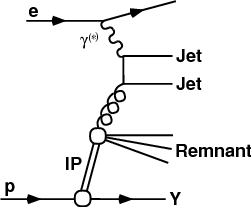
\includegraphics[width=2.2in]{Chapter2/importfigs/fig1a.png}
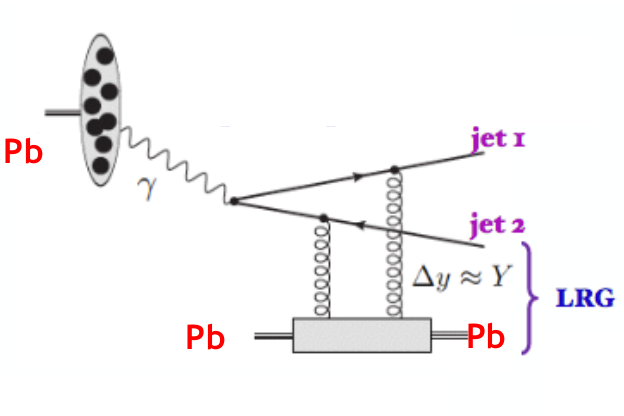
\includegraphics[width=3in]{Chapter2/importfigs/fig3_daniel_upc.png}
\par\end{centering}
\end{figure}

In electron-hadron collisions, diffractive photoproduction is characterized by the presence of a large rapidity gap in the final state and an intact nucleus. The Feynman diagram of electroproduction in lepton-hadron collisions is similar to that of photoproduction in ultraperipheral collisions. The diffractive dijet cross section is expressed by the convolution of partonic cross sections $d\hat{\sigma}$ and diffractive PDFs $f^D_{i/p}$.

\begin{equation}
d\sigma (ep \rightarrow e + 2 jets + X^{'} + p) = \sum_{i} \int dt \int dx_\mathbb{P} \int dz_\mathbb{P} d\hat{\sigma}_{ei\rightarrow 2jets}(\hat{s},\mu^2_R,\mu^2_F)\times f^D_{i/p}(z_\mathbb{P},\mu^2_F,x_\mathbb{P},t)
\end{equation}

In proton vertex factorisation, the dependence on $x_{\mathbb{P}}$ and $|t|$ is factored into a dependence on $\mu^2_F$ and $z_{\mathbb{P}}$.

\begin{equation}
f^D_{i/p}(z_{\mathbb{P}},\mu^2_F,x_{\mathbb{P}},t) = f_{\mathbb{P}/p}(x_{\mathbb{P}},t)f_{i/\mathbb{P}}(z_{\mathbb{P}},\mu^2_F) + n_\mathbb{R}f_{\mathbb{R}/p}(x_{\mathbb{P}},t)f_{i/\mathbb{R}}(z_{\mathbb{P}},
\mu^2_F) 
\end{equation}

Lepton-hadron collisions were performed at DESY and measured by the H1 and HERA experiments. These experiments reported a value for the total diffractive photoproduction cross section that is double that predicted by QCD collinear factorization. Diffractive events were selected for using rapidity gaps or the presence of leading protons in the very forward proton spectrometer (VFPS). 

\begin{figure}[h!]
\begin{centering}
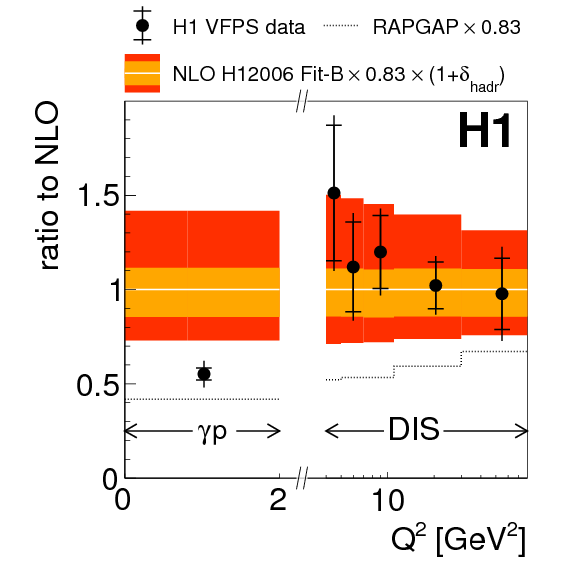
\includegraphics[width=3in]{Chapter2/importfigs/fig8_h1_2015.png}
\par\end{centering}
\end{figure}

H1 used the Very Forward Proton Spectrometer (VFPS) to trigger on low $Q^2$ protons. The VFPS consists of two Roman Pots located 218 m and 222 m from the H1 interaction-point in the forward direction. The VFPS can detect protons scattered at very low transverse momentum, corresponding to $0.008 < x_{P} < 0.028$ and $|t|<0.6$. Each of the Roman Pots contains layers of scintillating fibers, which are covered by a layer of scintillator tiles. The fibers readout to photomultipliers, and the tiles both shield from radiation and trigger on protons. The track effiency of VFPS is a remarkable $96 \%$, and the background contamination is kept at $1 \%$ , making the detector excellent for studying diffractive events.

\begin{figure}[h!]
\begin{centering}
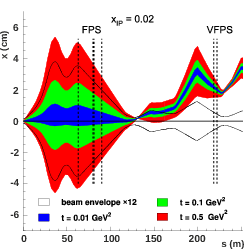
\includegraphics[width=3in]{Chapter2/importfigs/fig7_h1_2015.png}
\par\end{centering}
\end{figure}

The H1 data was compared to predictions based on NLO-QCD convoluted with diffractive parton distribution functions (DPDFs) from HERA inclusive diffractive deep-inelastic scattering (DDIS) data. For diffractive pp collisions the high transverse momentum jets yield a hard scale for perturbative QCD. 

\section{Wigner Distribution}

The quantum field theory lagrangian of the strong interaction is relatively simple, but because of confinement and asymptotic freedom the hadronic bound states are too complex for an analytic solution. Furthermore, collider experiment data requires a quantitative interpretation to be useful. The gap between QCD and heavy-ion data is bridged using the parton model, which considers hadrons as composed of quarks and gluons. Parton density functions (PDFs) model the longitudinal momentum distribution of the partons. PDFs are supplemented by transverse momentum distributions (TMDs) and generalized parton distributions (GPDs). In addition to transverse momentum, GPDs describe the transverse spatial distribution. TMDs and GPDs are derived from the final state particles of a collision. Markus Diehl maps the relationship between various distribution functions in figure X.

\begin{figure}[h!]
\begin{centering}
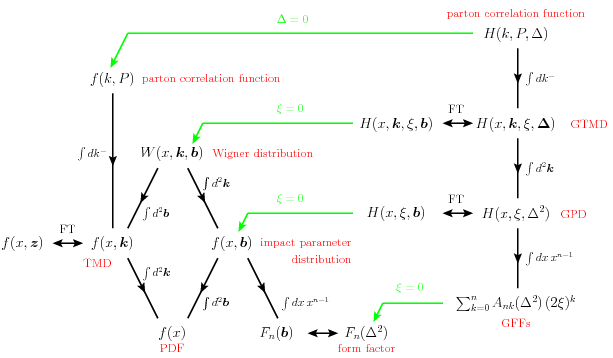
\includegraphics[width=7in]{Chapter2/importfigs/fig6_introGPD_TMD.png}
\par\end{centering}
\end{figure}

TMDs and GPDs manifest non-perturbative QCD effects. The Wigner distribution, at this scale, reflects the relationship between the position and momentum of partons.

\begin{figure}[h!]
\begin{centering}
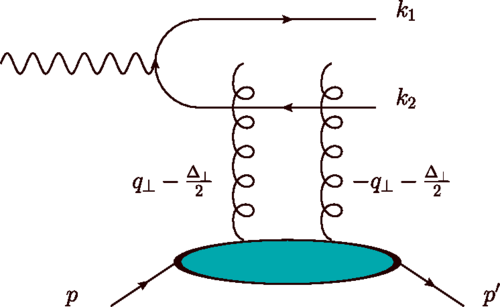
\includegraphics[width=4in]{Chapter2/importfigs/fig4_yatta.png}
\par\end{centering}
\end{figure}

Yoshitaka Hatta uses the dipole framework to show that the azimuthal angular correlations of coherent dijets are generated by the underlying gluon Wigner distribution. Furthermore, these correlations are consistent with predictions based on standard collinear factorization.

\begin{figure}[h!]
\begin{centering}
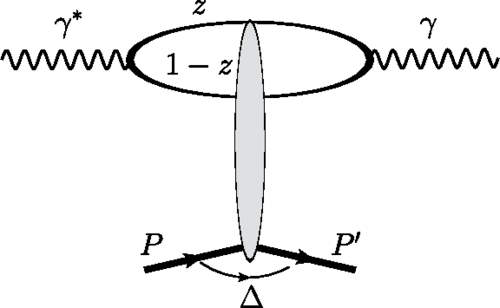
\includegraphics[width=4in]{Chapter2/importfigs/fig5_yatta_compton.png}
\par\end{centering}
\end{figure}

